\chapter{Implementacija i korisničko sučelje}
		
		
		\section{Korištene tehnologije i alati}
		
			\textbf{\textit{dio 2. revizije}}
			
			 \textit{Detaljno navesti sve tehnologije i alate koji su primijenjeni pri izradi dokumentacije i aplikacije. Ukratko ih opisati, te navesti njihovo značenje i mjesto primjene. Za svaki navedeni alat i tehnologiju je potrebno \textbf{navesti internet poveznicu} gdje se mogu preuzeti ili više saznati o njima}.
			
			
			\eject 
		
	
		\section{Ispitivanje programskog rješenja}
			
			\textbf{\textit{dio 2. revizije}}\\
			
			 \textit{U ovom poglavlju je potrebno opisati provedbu ispitivanja implementiranih funkcionalnosti na razini komponenti i na razini cijelog sustava s prikazom odabranih ispitnih slučajeva. Studenti trebaju ispitati temeljnu funkcionalnost i rubne uvjete.}
	
			
			\subsection{Ispitivanje komponenti}
			U ovom ćemo poglavlju predstaviti 9 ispitnih slučajeva (unit testova). Svi se ispitni primjeri mogu pronaći u datoteci janezi/izvorniKod/backend/common/tests.py koja je sastavljena od 4 klase koje ukupno sadrže 9 testova te sadrži 137 linija programskog koda.
			
			\vspace{5mm} %5mm vertical space
			
			Ispitni slučajevi 1 i 2 odnose se na prijavu korisnika. Oba se ispitna slučaja nalaze u klasi AccountTests. U prvom se slučaju korisnik ne može prijaviti jer mu korisnički račun nije potvrđen, dok se u drugom slučaju, odmah nakon potvrde računa, korisnik može uspješno prijaviti. U prvom je slučaju očekivan odgovor 400 (pogreška), dok je u drugom slučaju očekivan odgovor 200. Oba ispitna primjera daju očekivani rezultat.
			
			\begin{figure}[H]
				\centering
				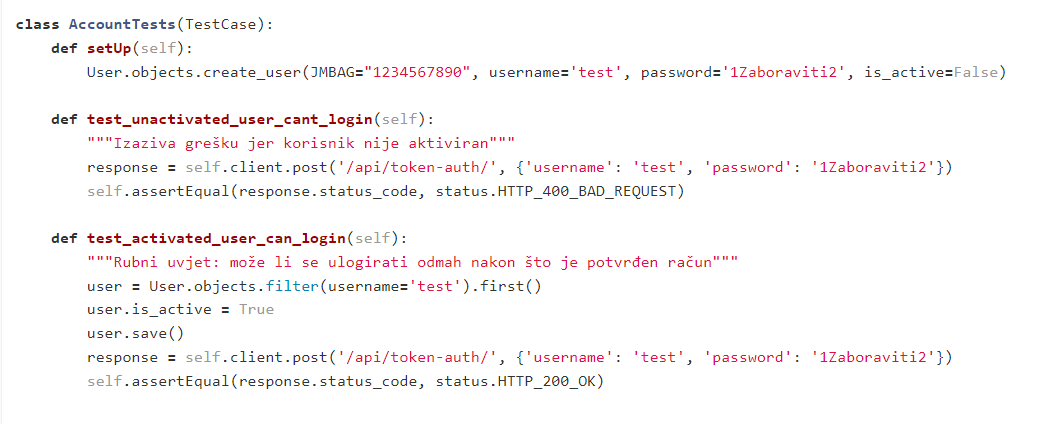
\includegraphics[scale=0.65]{slike/AccountTests.PNG}
				\caption{Ispitni slučajevi vezani za prijavu korisnika}
				\label{fig:promjene}
			\end{figure}
		
			Ispitni slučajevi 3 i 4 vezani su za administratora te provjeravaju ispravnost funkcionalnosti blokiranja korisnika. Oba se ispitna slučaja nalaze u klasi AdminTests. Prvi slučaj izaziva pogrešku (kod 401 UNAUTHORIZED) jer korisnik koji nije administrator pokušava blokirati račun drugog korisnika. U drugom slučaju, korisnik koji je administrator blokira korisnika i provjerava se točnost akcije. Oba ispitna primjera daju očekivani rezultat.
			
			\begin{figure}[H]
				\centering
				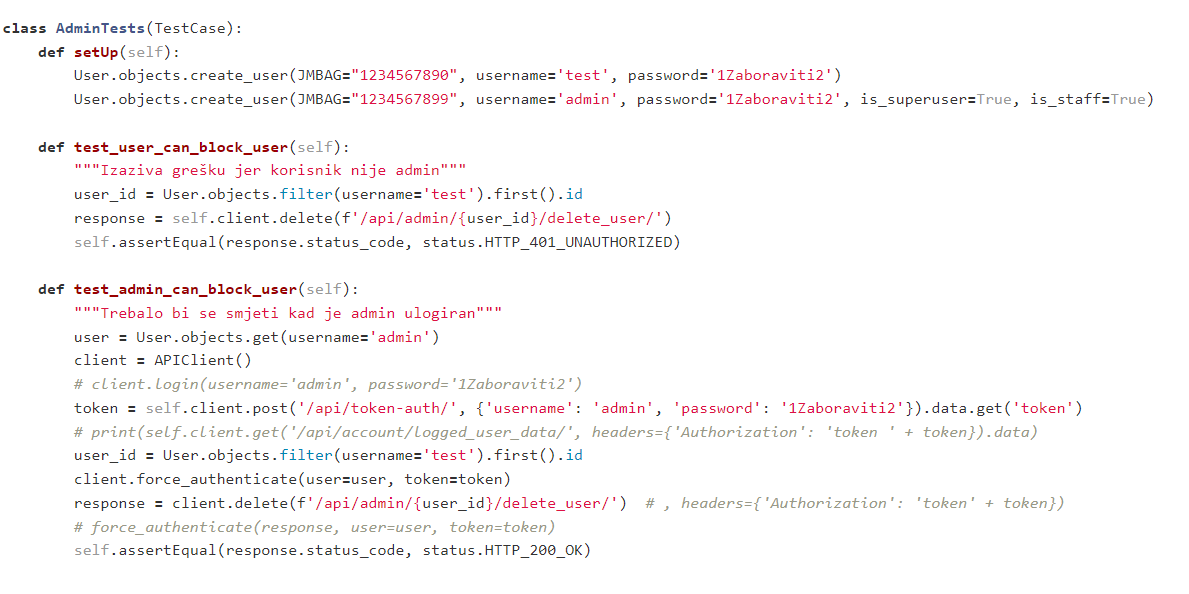
\includegraphics[scale=0.65]{slike/AdminTests.PNG}
				\caption{Ispitni slučajevi vezani za prijavu korisnika}
				\label{fig:promjene}
			\end{figure}
	
			Ispitni slučajevi 5, 6 i 7 odnose se na funkcionalnost vraćanja košare. Oba se ispitna slučaja nalaze u klasi WorkerTests. Prvi slučaj predstavlja situaciju u kojoj korisnik koji ne radi u praonici pokušava vratiti košaru. Taj bi slučaj trebao vratiti poruku 401 UNAUTHORIZED kako netko ne bi mogao zloupotrebljavati povrat košare. Drugi test provjerava ponašanje aplikacije u slučaju kad radnik pokuša označiti da je netko vratio košaru te osim provjere uspješnosti (kod 200), provjerava se i je li se broj košara tog korisnika smanjio na 0 (linija 75 u kodu). Sva tri ispitna primjera daju rezultat u skladu s očekivanjima.
			
			\begin{figure}[H]
				\centering
				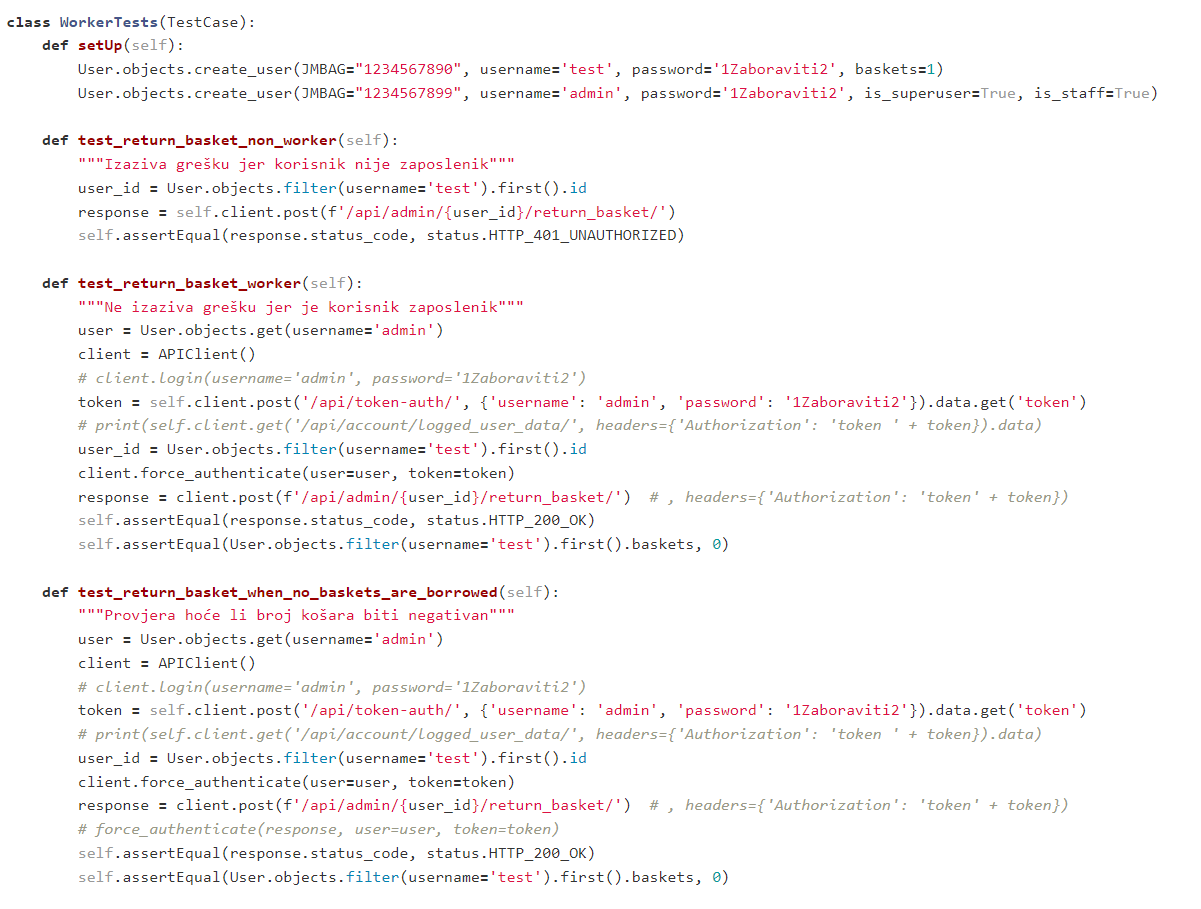
\includegraphics[scale=0.65]{slike/WorkerTests.PNG}
				\caption{Ispitni slučajevi vezani za vraćanje košara}
				\label{fig:promjene}
			\end{figure}
		
			Posljednja klasa ispitnih primjera, nalazi se u klasi AppointmentTests i sadrži ispitne primjere 8 i 9. Osmi ispitni primjer provjerava može li neregistrirani korisnik napraviti rezervaciju te je očekivano ponašanje pogreška s kodom 401. Ispitni primjer br. 9 ispituje rezervaciju termina nakon prijave i provjerava je li radnja bila uspješna (kod 201 CREATED). Oba ispitna primjera daju očekivani rezultat.
			
			\begin{figure}[H]
				\centering
				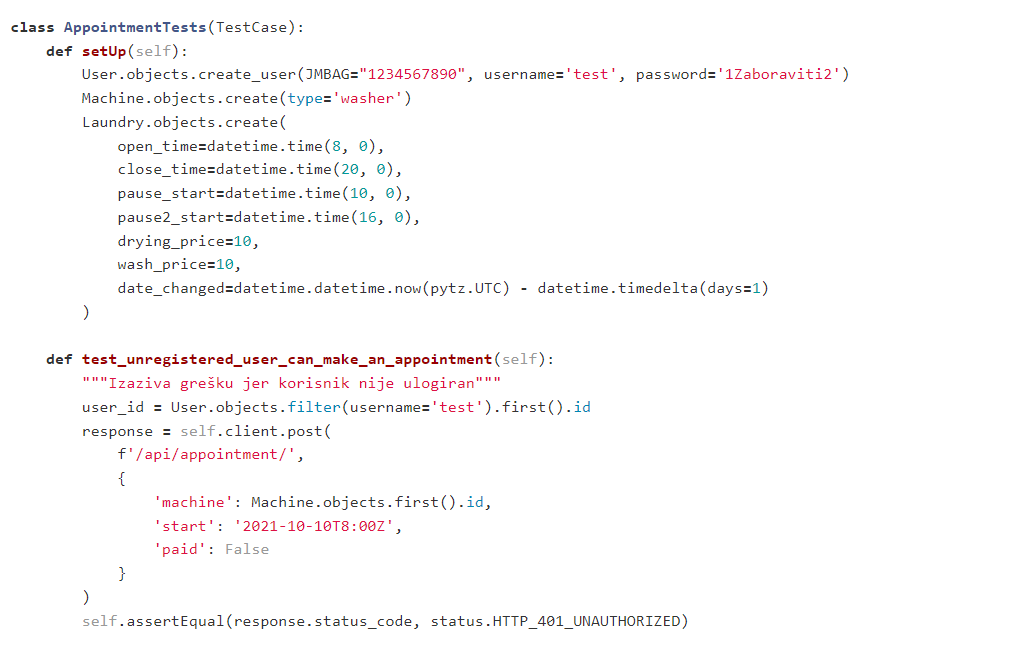
\includegraphics[scale=0.65]{slike/AppointmentTests1.PNG}
				\caption{Ispitni slučajevi vezani za rezervaciju termina, slika 1/2}
				\label{fig:promjene}
			\end{figure}
		
			\begin{figure}[H]
				\centering
				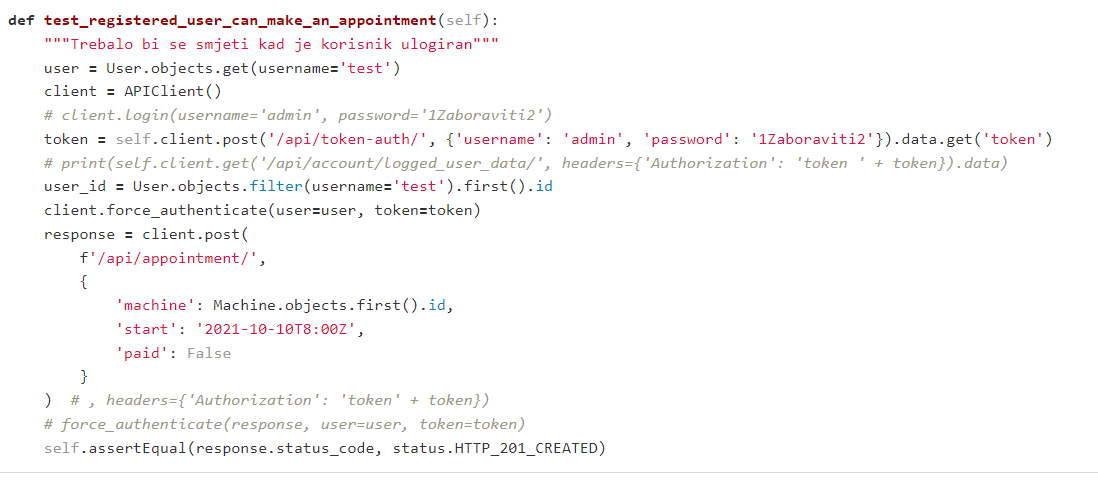
\includegraphics[scale=0.65]{slike/AppointmentTests2.PNG}
				\caption{Ispitni slučajevi vezani za rezervaciju termina, slika 2/2}
				\label{fig:promjene}
			\end{figure}
		
			Svi se spomenuti testovi mogu pokrenuti iz terminala aktivacijom virtualnog okruženja, pozicioniranjem u mapu backend i pozivanjem naredbe ./manage.py test. Kao što je već spomenuto, svi se testovi izvršavaju točno, a slika ~\ref{fig:TestsTerminal} pokretanja naredbe ./manage.py test dana je u prilogu. 
			
			\begin{figure}[H]
				\centering
				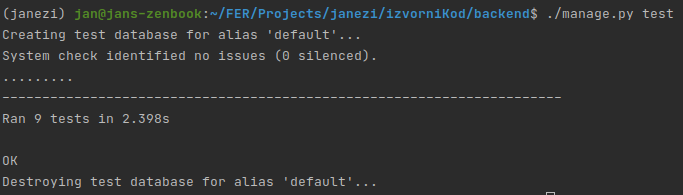
\includegraphics[scale=0.65]{slike/TestsTerminal.PNG}
				\caption{Pokretanje svih ispitnih slučajeva u terminalu}
				\label{fig:TestsTerminal}
			\end{figure}
			
			
			\subsection{Ispitivanje sustava}
			
			 \textit{Potrebno je provesti i opisati ispitivanje sustava koristeći radni okvir Selenium\footnote{\url{https://www.seleniumhq.org/}}. Razraditi \textbf{minimalno 4 ispitna slučaja} u kojima će se ispitati redovni slučajevi, rubni uvjeti te poziv funkcionalnosti koja nije implementirana/izaziva pogrešku kako bi se vidjelo na koji način sustav reagira kada nešto nije u potpunosti ostvareno. Ispitni slučaj se treba sastojati od ulaza (npr. korisničko ime i lozinka), očekivanog izlaza ili rezultata, koraka ispitivanja i dobivenog izlaza ili rezultata.\\ }
			 
			 \textit{Izradu ispitnih slučajeva pomoću radnog okvira Selenium moguće je provesti pomoću jednog od sljedeća dva alata:}
			 \begin{itemize}
			 	\item \textit{dodatak za preglednik \textbf{Selenium IDE} - snimanje korisnikovih akcija radi automatskog ponavljanja ispita	}
			 	\item \textit{\textbf{Selenium WebDriver} - podrška za pisanje ispita u jezicima Java, C\#, PHP koristeći posebno programsko sučelje.}
			 \end{itemize}
		 	\textit{Detalji o korištenju alata Selenium bit će prikazani na posebnom predavanju tijekom semestra.}
			
			\eject 
		
		
		\section{Dijagram razmještaja}
			
			\textbf{\textit{dio 2. revizije}}
			
			 \textit{Potrebno je umetnuti \textbf{specifikacijski} dijagram razmještaja i opisati ga. Moguće je umjesto specifikacijskog dijagrama razmještaja umetnuti dijagram razmještaja instanci, pod uvjetom da taj dijagram bolje opisuje neki važniji dio sustava.}
			
			\eject 
		
		\section{Upute za puštanje u pogon}
		
			\textbf{\textit{dio 2. revizije}}\\
		
			 \textit{U ovom poglavlju potrebno je dati upute za puštanje u pogon (engl. deployment) ostvarene aplikacije. Na primjer, za web aplikacije, opisati postupak kojim se od izvornog kôda dolazi do potpuno postavljene baze podataka i poslužitelja koji odgovara na upite korisnika. Za mobilnu aplikaciju, postupak kojim se aplikacija izgradi, te postavi na neku od trgovina. Za stolnu (engl. desktop) aplikaciju, postupak kojim se aplikacija instalira na računalo. Ukoliko mobilne i stolne aplikacije komuniciraju s poslužiteljem i/ili bazom podataka, opisati i postupak njihovog postavljanja. Pri izradi uputa preporučuje se \textbf{naglasiti korake instalacije uporabom natuknica} te koristiti što je više moguće \textbf{slike ekrana} (engl. screenshots) kako bi upute bile jasne i jednostavne za slijediti.}
			
			
			 \textit{Dovršenu aplikaciju potrebno je pokrenuti na javno dostupnom poslužitelju. Studentima se preporuča korištenje neke od sljedećih besplatnih usluga: \href{https://aws.amazon.com/}{Amazon AWS}, \href{https://azure.microsoft.com/en-us/}{Microsoft Azure} ili \href{https://www.heroku.com/}{Heroku}. Mobilne aplikacije trebaju biti objavljene na F-Droid, Google Play ili Amazon App trgovini.}
			
			
			\eject 